\documentclass[tikz, border=10pt]{standalone}
\usepackage{tikz}
\usetikzlibrary{calc}

\begin{document}

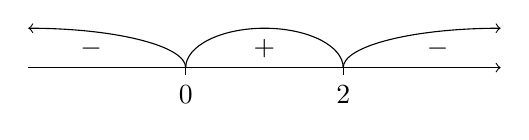
\begin{tikzpicture}
    \draw[->] (-2,0) to (4,0);

    \foreach \x in {0,2} {
        \draw (\x,0.02) to (\x,-0.1) node[below] {$\x$};
    }

    \draw (0,0) arc[x radius=1, y radius=0.5, start angle=180, end angle=0];
    \draw[->] (2,0) arc[x radius=2, y radius=0.5, start angle=180, end angle=90];
    \draw[->] (0,0) arc[x radius=2, y radius=0.5, start angle=0, end angle=90];

    \node[above] at (-1.2,0) {$-$};
    \node[above] at (1,0) {$+$};
    \node[above] at (3.2,0) {$-$};
\end{tikzpicture}

\end{document}
